\documentclass[11pt,conference]{IEEEtran}
\IEEEoverridecommandlockouts

\usepackage[utf8]{inputenc}
\usepackage[T1]{fontenc}
\usepackage{amsmath,amssymb,amsfonts}
\usepackage{graphicx}
\usepackage{cite}
\usepackage{booktabs}
\usepackage{array}
\usepackage{url}
\usepackage{balance}
\usepackage[letterpaper,top=0.75in,bottom=1.10in,left=0.75in,right=0.75in]{geometry}
\setlength{\columnsep}{0.25in}
\setlength{\textfloatsep}{7pt plus 2pt minus 2pt}
\setlength{\floatsep}{6pt plus 2pt minus 2pt}
\setlength{\dbltextfloatsep}{7pt plus 2pt minus 2pt}
\setlength{\dblfloatsep}{6pt plus 2pt minus 2pt}

% Configure graphics search path for publication assets
\graphicspath{{figures/}}

\title{Turn-Aware Search and Road-Impedance Modelling for Two-Wheeler Routing in Urban Road Networks}

\author{
\IEEEauthorblockA{
\textbf{Anirudh R}\\
Dept. of CSE\\
BNM Institute of Technology\\
Bengaluru, India\\
\texttt{anirudhraju7@gmail.com}\\[4pt]
\textbf{Vikhyath K B}\\
Dept. of CSE\\
BNM Institute of Technology\\
Bengaluru, India\\
\texttt{vikhyathkb@bnmit.in}\\[4pt]
\textbf{A Nikhil Kumar}\\
Dept. of CSE\\
BNM Institute of Technology\\
Bengaluru, India\\
\texttt{23cse100@bnmit.in}}
\and
\IEEEauthorblockA{
\textbf{Shwetha M D}\\
Dept. of CSE\\
BNM Institute of Technology\\
Bengaluru, India\\
\texttt{shwetha.0116@gmail.com}\\[4pt]
\textbf{Akshath G}\\
Dept. of CSE\\
BNM Institute of Technology\\
Bengaluru, India\\
\texttt{23cse167@bnmit.in}\\[4pt]
\textbf{Chiranandan T M}\\
Dept. of CSE\\
BNM Institute of Technology\\
Bengaluru, India\\
\texttt{23cse186@bnmit.in}}
}

\begin{document}

\maketitle

\begin{abstract}
Vertex-based shortest-path routing does not directly represent arrival heading or turn-dependent costs. This paper presents a two-wheeler routing method combining state-expanded $A^*$ search, discrete angular penalties, and road-class impedance. States are directed edges $s=(u,v)$; qualifying grade-separated main-road edges receive a $0.80$ multiplier. When all edge multipliers satisfy $\mu(e)\ge0.80$ and turn penalties are nonnegative, a Haversine heuristic scaled by $0.80$ is admissible and consistent. Evaluation on 25 Bengaluru origin--destination corridors (744,216 directed edge records) shows that turn-aware routing (A0) reduces mean sharp turns by $34.1\%$ versus turn-unaware state expansion (A1; 32.52 to 21.44; Holm-adjusted $p=4.5\times10^{-5}$). Production impedance (B0) reduces arterial exposure by 51.21 percentage points versus neutral weights (B1; 65.05\% to 13.84\%), with a 15.53\% increase in mean physical route distance (7.65 versus 6.62 km). The results quantify the effects of turn costs and road-class impedance; they do not establish real-world travel-time or safety benefits.
\end{abstract}

\begin{IEEEkeywords}
Two-wheeler routing, state-expanded search, turn penalties, shortest path algorithms, road impedance modeling, heuristic admissibility, urban transportation networks.
\end{IEEEkeywords}

\section{Introduction}

Indian metropolitan traffic includes substantial two-wheeler use, with operating conditions distinct from passenger cars \cite{promraksa2022lane,kotagi2020modeling}. In dense networks such as Bengaluru, riders encounter frequent intersections, grade changes, and acute turns. Commercial routing commonly prioritizes passenger automobiles and may omit vehicle-specific impedance and turn effort \cite{kumar2025realtime}, potentially directing two-wheelers toward arterial corridors or routes with frequent turns.

Conventional routing evaluates link distance or travel-time costs at graph vertices \cite{luxen2011realtime}. This node-centric model cannot directly represent a turn because traversal of outbound edge $(v,w)$ depends on inbound edge $(u,v)$ \cite{das2019modeling,winter2002modeling}. State expansion addresses this by representing directed edges, rather than intersections, as search states \cite{kirby1969minimum}.

Turn penalties depend on inbound approach and outbound heading, motivating edge-expanded representations that map vertices to directed-edge states \cite{winter2002modeling,kirby1969minimum}. Contraction Hierarchies (CH) and Customizable Contraction Hierarchies (CCH) also support turn costs \cite{geisberger2011efficient,bast2016route}; however, heterogeneous road-class and topological metrics can increase customization and shortcut complexity \cite{bast2016route}.

Road class can affect two-wheeler route suitability. Prior studies examine motorcycle responses to traffic information and multi-criteria route assessment \cite{fadilah2024identifying,asvial2020entropy}; configured weights nevertheless require independent behavioral calibration.

We combine turn-aware state-expanded $A^*$ with road-class impedance, evaluating angular penalties during edge relaxation without materializing a line graph. A $0.80$ override applies to qualifying grade-separated main-road edges. We establish conditional admissibility and consistency of a Haversine heuristic scaled by $0.80$ when $\mu(e)\ge0.80$ and turn penalties are nonnegative \cite{hart1968formal}. Across 25 Bengaluru corridors, A0 reduces sharp turns by 34.1\% versus A1 (21.44 versus 32.52; adjusted $p=4.5\times10^{-5}$); B0 reduces arterial exposure by 51.21 percentage points versus B1, with 15.53\% greater mean physical distance.

Section II reviews related work; Sections III--IV present the model, algorithm, correctness conditions, and complexity; Sections V--VI describe and evaluate Experiments A--D; Section VII concludes.

\section{Related Work}

\noindent\textbf{Shortest-Path Routing and Turn-Aware State Representations:} Early work showed that turn penalties require expanded network representations rather than independent vertex costs \cite{kirby1969minimum}. Winter formalized directed edge-to-edge transitions through line- and dual-graph models; this preserves standard shortest-path methods but increases state and transition counts on dense networks \cite{winter2002modeling}.

\noindent\textbf{Hierarchical Routing and Metric Customization:} Contraction Hierarchies and Customizable Contraction Hierarchies accelerate large-scale routing and can incorporate turn costs through node expansion and turn-aware ordering \cite{geisberger2011efficient,bast2016route,delling2017customizable}. Their metric customization must be repeated when vehicle profiles or cost functions change, adding operational complexity for heterogeneous urban costs.

\noindent\textbf{Two-Wheeler Trajectory Analysis and Rider Preference:} Two-wheeler traffic involves speed dispersion and queue lane-filtering \cite{kotagi2020modeling,promraksa2022lane}. Fadilah et al. used stated-preference modelling and microscopic simulation to study motorcycle route selection under traffic-information scenarios in Ninh Ki\^{e}u District, Vietnam \cite{fadilah2024identifying}. Asvial et al. generated candidate routes without turn penalties and applied post-hoc Entropy-TOPSIS ranking \cite{asvial2020entropy}. Here, configured impedance is evaluated within graph search as an engineering cost, not as calibrated rider preference.

\noindent\textbf{Research Positioning and Synthesis:} Prior work uses line graphs, hierarchical indexing, or post-hoc motorcycle route ranking \cite{winter2002modeling,geisberger2011efficient,asvial2020entropy,zografos2004heuristic,kumar2025realtime}. We integrate turn penalties and road-class impedance in edge-state search and establish conditional consistency of the scaled Haversine heuristic.

\section{Problem Formulation and Configured Road Impedance}

\noindent\textbf{Directed Road-Network and Routing Problem:} The Bengaluru network is a directed multigraph $G_{\mathrm{raw}}=(V,E_{\mathrm{raw}})$ with $|V|=308{,}643$ and $744{,}216$ raw edge records. Of these, 3,379 ordered pairs contain parallel edges (6,773 records; maximum multiplicity four). Search collapses each pair to its minimum-impedance representative, yielding $G=(V,E_s)$ with $|E_s|=740{,}822$. For $(u,v)\in E_s$, $c_{\min}(u,v)=\min_{k\in\mathcal{K}(u,v)}[\mu(u,v,k)\ell(u,v,k)]$, where $\ell>0$ is physical length and $\mu$ the composite multiplier. Given origin $s_0$ and destination $t$, the algorithm minimizes path impedance $C(P)$ in effective metres; physical distance $D(P)=\sum_i\ell(e_i)$ remains distinct from impedance, travel time, and congestion.

\noindent\textbf{Edge-Based State Representation:} Turn costs depend on the inbound trajectory, so states are directed edges $s=(u,v)$ representing arrival at $v$ from $u$. Parallel edges use $c_{\min}(u,v)$ and carry no separate state key. Origin departure uses synthetic state $(\mathrm{None},s_0)$; thus $S=E_s\cup\{(\mathrm{None},s_0)\}$ contains 740,823 states. A transition from $(u,v)$ to $(v,w)$ is valid when $(v,w)\in E_s$.

\noindent\textbf{Angular Turn-Deflection Model:} For inbound $(u,v)$ and outbound $(v,w)$ segments, let $\theta(u,v)$ and $\theta(v,w)$ be initial forward azimuths from endpoint coordinates. Their smaller angular difference defines $\Delta\theta(u,v,w)$:
\begin{equation*}
\begin{aligned}
\Delta\theta(u,v,w) = \min\{&
|\theta(u,v)-\theta(v,w)|,\\
&360^\circ-|\theta(u,v)-\theta(v,w)|\},\\
&\Delta\theta\in[0^\circ,180^\circ].
\end{aligned}
\end{equation*}
Internal roadway polyline shape points are not evaluated. Turning penalties are assigned by a discrete piecewise function:
\begin{equation}
\label{eq:turn_penalty}
P_{\text{turn}}(u,v,w)=
\begin{cases}
25.0, & u\ne\mathrm{None},\ \Delta\theta\ge60^\circ,\\
8.0, & \substack{u\ne\mathrm{None},\\30^\circ\le\Delta\theta<60^\circ},\\
0.0, & \text{otherwise}.
\end{cases}
\end{equation}
Penalties are 25 and 8 effective metres for sharp ($\ge60^\circ$) and moderate ($30^\circ$--$60^\circ$) deflections; smaller deflections and origin departure incur zero cost. These terms measure geometric deflection, not cross-traffic conflict or collision risk.

\noindent\textbf{Configured Road-Impedance Model and Objective Function:} To incorporate vehicle-specific street hierarchy weighting into graph traversal, edge segments receive a composite multiplier $\mu(e)$:
\begin{equation}
\label{eq:road_impedance}
\mu(e)=
\begin{cases}
0.80\,m_{\mathrm{rbt}}(e), &
\substack{\text{bridge}(e)\in\mathcal{B}^{+},\\
h(e)\in\mathcal{H}_{\mathrm{main}}},\\
f_{\mathrm{class}}(h(e))\,m_{\mathrm{rbt}}(e), & \text{otherwise}.
\end{cases}
\end{equation}
Here, $\mathcal{B}^+$ marks affirmative bridge tags, $\mathcal{H}_{\mathrm{main}}$ qualifying main roads, and $m_{\mathrm{rbt}}=0.95$ for roundabouts (otherwise 1.0). Table~\ref{tab:road_impedance} lists class weights and modifiers. A qualifying bridge replaces the base weight with 0.80; the roundabout factor is then applied, so a hypothetical co-occurrence yields 0.76. No such co-occurrence occurs in the 744,216-edge corpus; the observed minimum is 0.80. Thus $\mu(e)\ge0.80$ is verified for this graph, not asserted universally.

For state transition $s = (u, v)$ to $s' = (v, w)$ over $E_s$, the traversal cost and path objective are:
\begin{equation}
\label{eq:path_objective}
\begin{aligned}
c(s, s') &= c_{\min}(v, w) + P_{\text{turn}}(u, v, w) \\
C(P) &= \sum_{i=1}^k c_{\min}(v_{i-1}, v_i) + \sum_{i=1}^{k-1} P_{\text{turn}}(v_{i-1}, v_i, v_{i+1})
\end{aligned}
\end{equation}
$C(P)$ charges each edge once through $c_{\min}$ and each intermediate turn once; origin departure and destination termination have zero turn penalty.

\begin{table*}[t]
\caption{Configured Road-Class Impedance Multipliers and Topological Modifiers}
\label{tab:road_impedance}
\centering
\small
\begin{tabular*}{\textwidth}{@{\extracolsep{\fill}}>{\raggedright\arraybackslash}p{1.05in}>{\raggedright\arraybackslash}p{1.40in}>{\raggedright\arraybackslash}p{2.35in}>{\raggedright\arraybackslash}p{1.00in}@{}}
\hline
\textbf{Hierarchy Category} & \textbf{OSM Classification ($h(e)$)} & \textbf{Modifier Condition} & \textbf{Effective Multiplier ($\mu$)} \\
\hline
\multicolumn{4}{l}{\textit{Part A: Base Road-Class Impedance ($f_{\mathrm{class}}$)}} \\
Arterial Trunk / Highway & \texttt{motorway}, \texttt{trunk} & Standard surface & $3.00\text{--}4.00$ \\
Primary Corridor & \texttt{primary}, \texttt{primary\_link} & Standard surface & $2.00\text{--}2.20$ \\
Secondary Corridor & \texttt{secondary}, \texttt{secondary\_link} & Standard surface & $1.40\text{--}1.50$ \\
Intermediate Collector & \texttt{tertiary}, \texttt{tertiary\_link} & Standard surface & $1.10\text{--}1.15$ \\
Local / Residential & \texttt{residential}, \texttt{unclassified} & Neutral baseline & $1.00$ \\
Permissive Street & \texttt{living\_street}, \texttt{service} & Standard surface & $0.90\text{--}0.95$ \\
\hline
\multicolumn{4}{l}{\textit{Part B: Topological Modifiers}} \\
Grade-Separated Flyover & $\mathcal{H}_{\mathrm{main}}$ on bridge structure & Replaces $f_{\mathrm{class}}$ with $0.80$ & $0.80$ \\
Continuous-Flow Roundabout & All classes tagged as roundabouts & Scales base by $\times 0.95$ & $0.95 \cdot f_{\mathrm{class}}$ (down to $0.855$) \\
Theoretical Co-occurrence & $\mathcal{H}_{\mathrm{main}}$ bridge $+$ roundabout & $0.80 \times 0.95$ ($0$ in corpus) & $0.76$ \\
\hline
\end{tabular*}
\end{table*}

\section{Turn-Aware $A^*$ Algorithm, Correctness and Complexity Analysis}

\noindent\textbf{A. Turn-Aware State-Expanded Search Architecture:} Search operates directly on edge states. From $(u,v)$ it generates successors $(v,w)$, using $c_{\min}(v,w)$ for parallel edges and transition cost $c(s,s')=c_{\min}(v,w)+P_{\mathrm{turn}}(u,v,w)$. A synthetic origin state incurs no departure penalty. A binary min-heap orders states by $(g+h,\kappa,s)$; strict improvements update costs and backpointers. The first extracted destination state terminates search and yields the reconstructed path.

\noindent\textbf{B. Scaled Haversine Heuristic Formulation:} For destination $t$, the Haversine distance underestimates physical path length. With edge multipliers bounded below by $\mu_{\min}=0.80$, the cost heuristic is:
\begin{equation}
\label{eq:scaled_heuristic}
h(s) = \mu_{\min} \cdot D_{\text{haversine}}(v, t) = 0.80 \cdot D_{\text{haversine}}(v, t)
\end{equation}
The lower bound corresponds to qualifying grade-separated main-road edges; ordinary surface edges have multipliers at least 1.0.

\noindent\textbf{C. Heuristic Admissibility and Consistency:} The proof assumes $\mu(e)\ge0.80$, nonnegative turn penalties, edge length at least its endpoint Haversine distance, and the spherical triangle inequality. Therefore:
\begin{equation}
\label{eq:consistency_condition}
h(s) \le c(s,s') + h(s')
\end{equation}
The triangle inequality gives $h(s)\le0.80D_{\mathrm{haversine}}(v,w)+h(s')$. The edge-cost lower bound and nonnegative turn penalty then give $h(s)\le c(s,s')+h(s')$. The heuristic is consistent and admissible; first extraction is optimal, so reopening is unnecessary.

\noindent\textbf{D. Computational Complexity Analysis:} Search uses $|E_s|+1$ states. Without decrease-key, improvements push duplicate heap entries; successor evaluation may inspect up to $q_{\max}$ parallel candidates. General directed-graph bounds are:
\begin{equation}
\label{eq:complexity_bounds}
\begin{aligned}
\mathcal{T}_{\text{general}} &= \mathcal{O}\bigl(
|E_s|d_{\max}^{\text{out}}\log(|E_s|d_{\max}^{\text{out}})\\
&\qquad + q_{\max}|E_s|d_{\max}^{\text{in}}d_{\max}^{\text{out}}\bigr),\\
\mathcal{M}_{\text{general}} &= \mathcal{O}(|E_s|d_{\max}^{\text{out}}+|V|).
\end{aligned}
\end{equation}
With bounded degree and multiplicity, time is $\mathcal{O}(|E_s|\log|E_s|)$ and logical memory is $\mathcal{O}(|E_s|)$. Bengaluru maxima ($d^{in}=d^{out}=6$, $q_{\max}=4$) imply saturation bounds of 5,886,792 successor iterations and 3,877,450 logical entries; observed queries used 119--129,619 queue pops (median 174.93 ms).

\section{Experimental Setup and Methodology}

\subsection{Urban Road Network and OD Corridor Corpus}

Evaluation uses a directed OpenStreetMap network of Bengaluru (308,643 vertices; 744,216 raw edges; 740,822 distinct ordered pairs) and 25 origin--destination corridors. Reference-route distances range from 1.35 to 15.82 km; the corridor is the analysis unit.

\subsection{Benchmark Configurations and Execution Protocol}

Four suites compare: A, turn-aware, turn-unaware, and node-level search; B, production impedance, neutral weights, and physical shortest paths; C, four turn-penalty tiers; and D, bridge/roundabout modifiers in a $2\times2$ design. Each of 350 corridor--configuration cells has five repetitions (1,750 observations); wall-clock runtime uses \texttt{time.perf\_counter()}.

\subsection{Statistical Analysis}

Five-run medians are paired by corridor ($N=25$). Two-sided Wilcoxon signed-rank tests use Pratt zero correction and Holm--Bonferroni family-wise adjustment. Reported effect sizes are matched-pairs Cohen's $d_z$ and Hodges--Lehmann paired median differences, with 95\% confidence intervals.

\section{Experimental Results and Discussion}

\subsection{Turn Awareness and State-Expansion Trade-offs}

In Experiment A (Fig.~\ref{fig:exp_a_tradeoffs}), A0 reduces mean sharp turns ($\ge60^\circ$) from 32.52 (A1) to 21.44: a 34.1\% reduction (mean difference $-11.08$, $W=0$, adjusted $p=4.5\times10^{-5}$, $d_z=-1.0066$, Hodges--Lehmann $-9.50$). A1 and node-level A2 have identical turn counts, geometry, and physical distances on all 25 corridors (mean difference 0; 7.723 km; descriptive invariance, not an inferential distance test).

Median runtime was 154.69 ms for A1 and 174.93 ms for A0 (+13.1\%; mean paired difference +41.35 ms, adjusted $p=1.2\times10^{-5}$, $d_z=0.7947$). A1 was 3.78 times slower than node-level A2 (154.69 vs. 40.88 ms; adjusted $p<10^{-6}$, $d_z=0.8115$). A0 corridor medians ranged from 1.01 to 1,829.18 ms (mean 382.98, SD 464.48, median 174.93, IQR 439.08); sub-second runtime was not universal.

\begin{figure}[t]
\centering
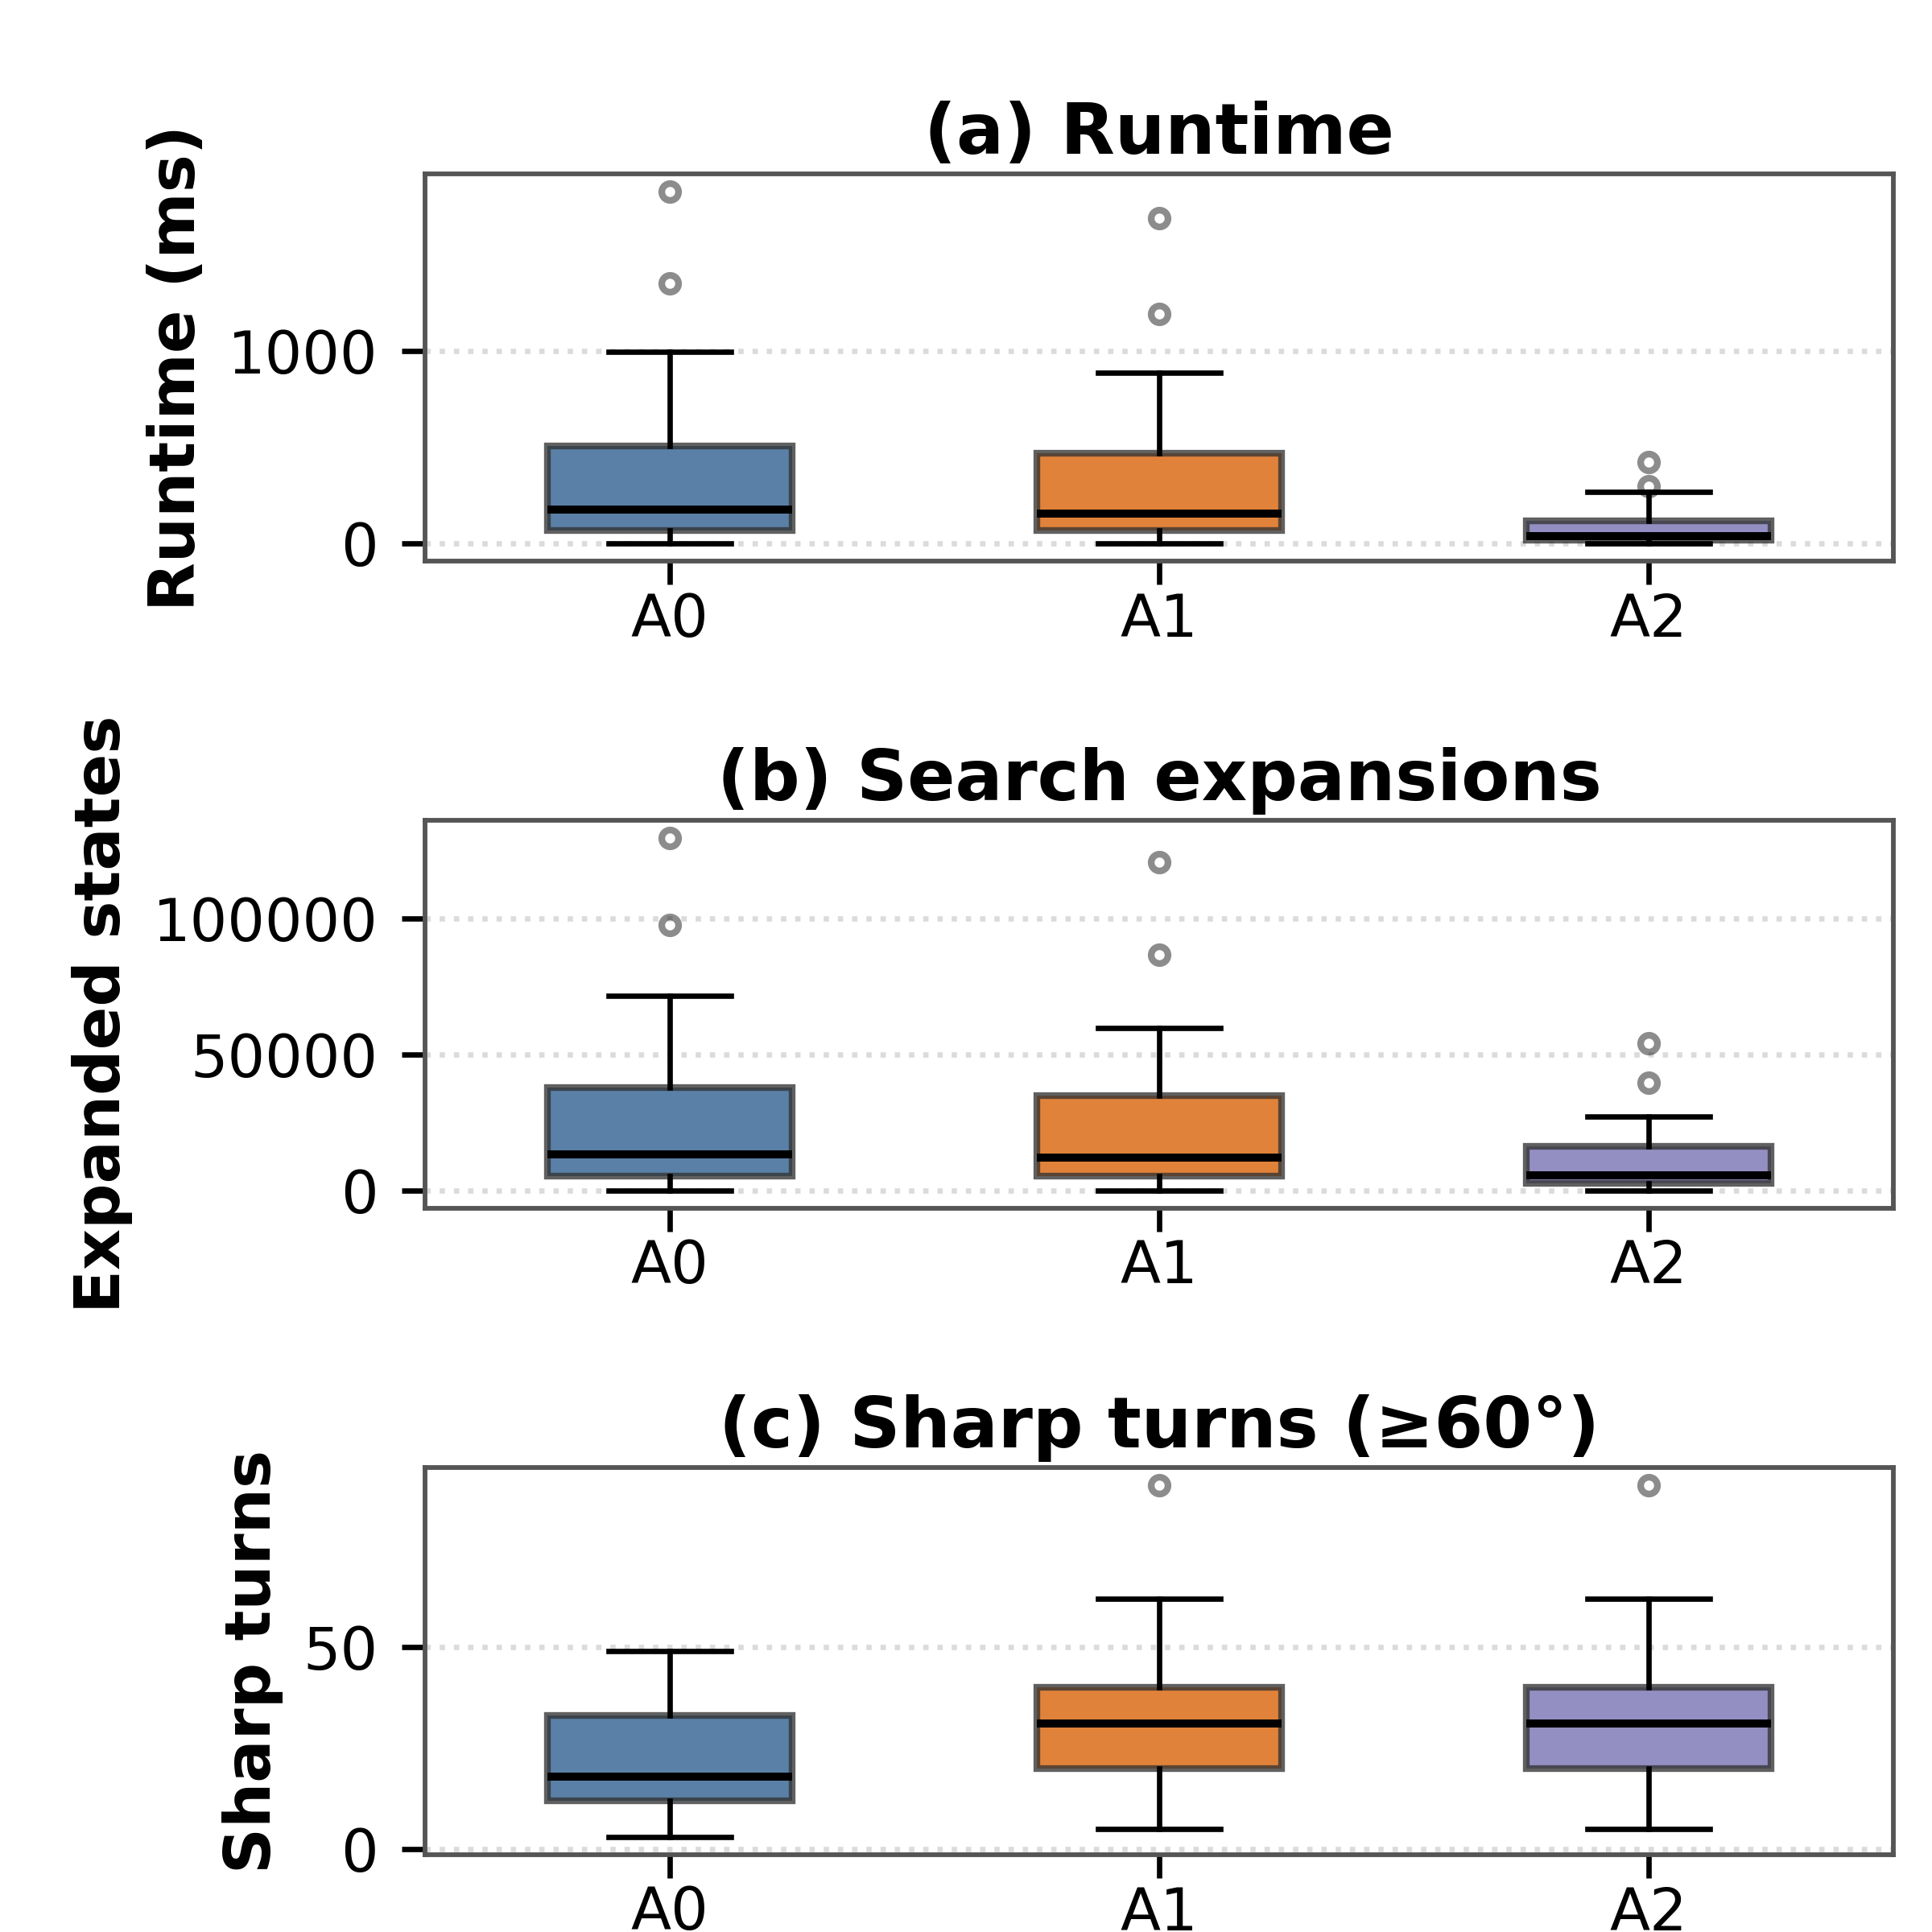
\includegraphics[width=\columnwidth]{fig1_exp_a_tradeoffs.png}
\caption{Experiment A distributions across 25 corridors: (a) wall-clock runtime, (b) expanded search states, and (c) sharp-turn counts ($\ge 60^\circ$) for turn-aware ($A_0$), turn-unaware state-expanded ($A_1$), and node-level ($A_2$) routing.}
\label{fig:exp_a_tradeoffs}
\end{figure}

\subsection{Road-Class Impedance and Street-Hierarchy Allocation}

In B0 (Fig.~\ref{fig:exp_b_road_classes}), arterial exposure falls from 65.05\% (B1) to 13.84\% (-51.21 percentage points; $W=4$, adjusted $p=8.4\times10^{-5}$, $d_z=-1.7715$, Hodges--Lehmann -54.55\%). Residential share rises from 13.51\% to 44.24\% (+30.73 points; $W=9$, adjusted $p=1.5\times10^{-4}$, $d_z=1.5234$, Hodges--Lehmann +31.30\%). Mean physical distance increases from 6.620 to 7.647 km (+15.53\%, +1.028 km; $W=7$, adjusted $p=6.8\times10^{-5}$, $d_z=0.9246$, Hodges--Lehmann +0.86 km). Versus shortest-distance B2 (59.35\% arterial), B0 reduces arterial exposure by 45.51 points (adjusted $p=8.4\times10^{-5}$, $d_z=-1.5862$, Hodges--Lehmann -46.31\%). Impedance is not physical distance or travel time.

\begin{figure}[t]
\centering
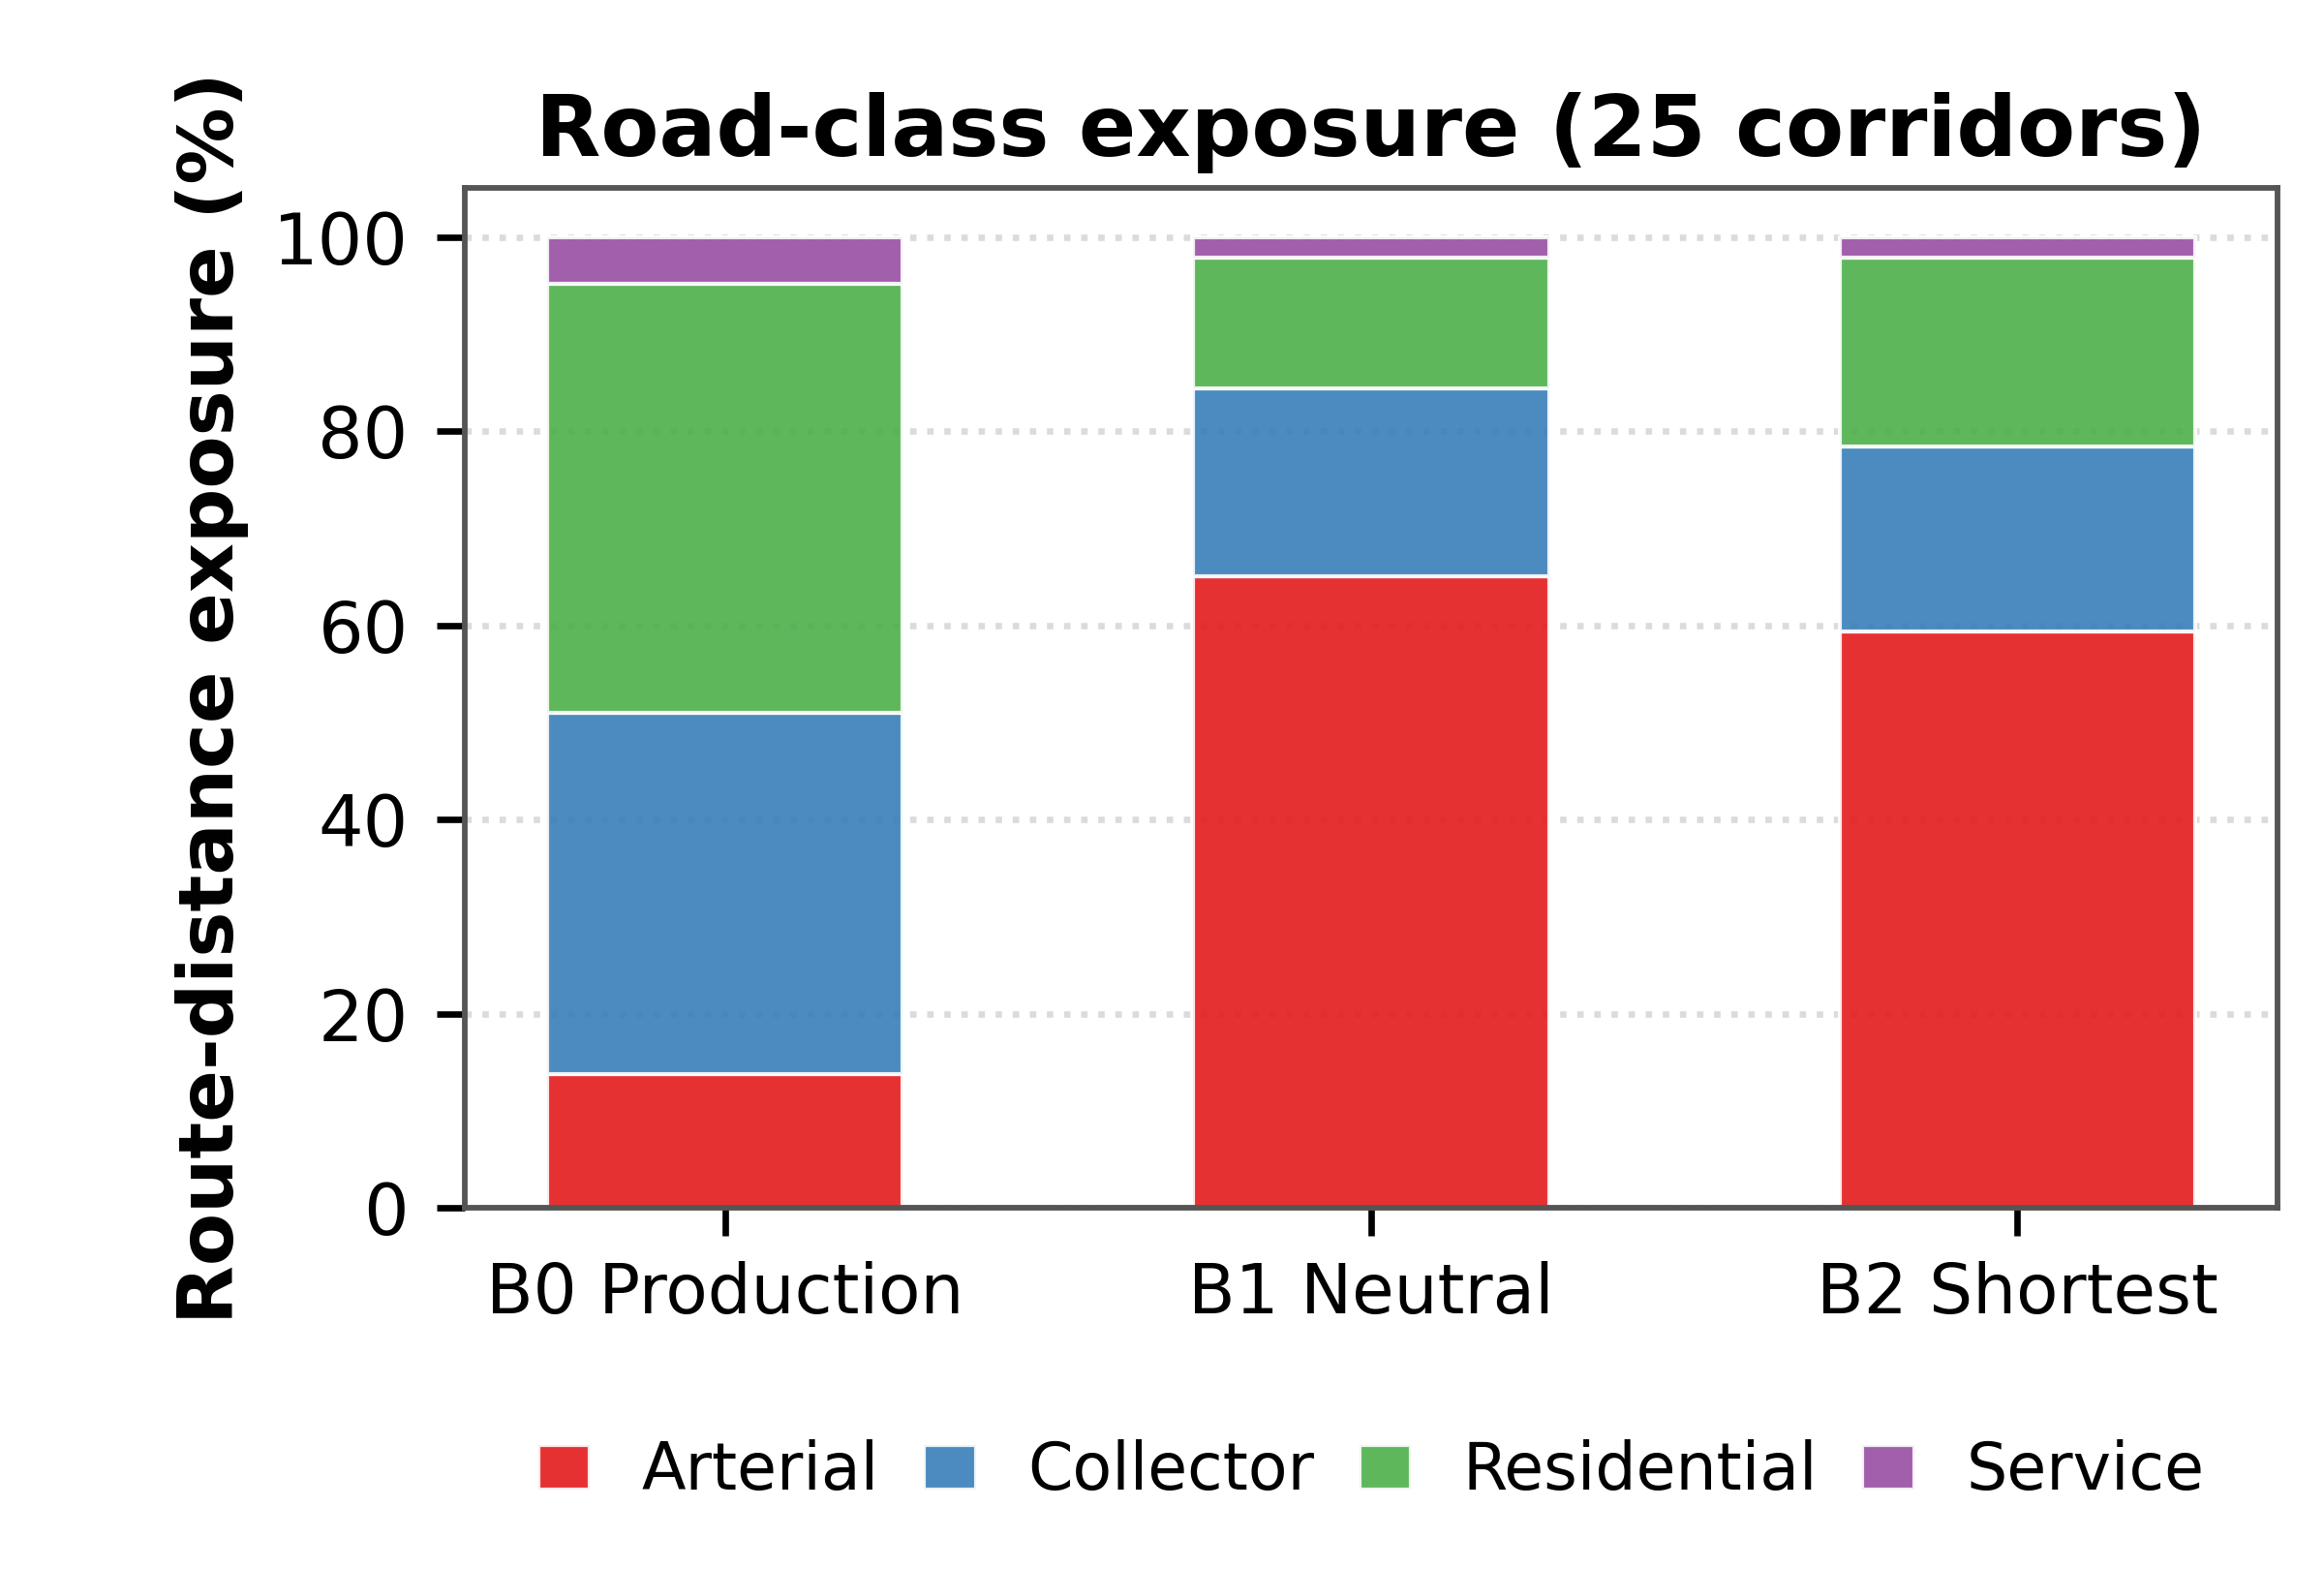
\includegraphics[width=\columnwidth]{fig2_exp_b_road_classes.png}
\caption{Experiment B mean route-distance exposure by road class across 25 corridors for production impedance ($B_0$), neutral road-class weights ($B_1$), and physical shortest-distance routing ($B_2$). Stacked bars show arterial, collector, residential, and service shares.}
\label{fig:exp_b_road_classes}
\end{figure}

\subsection{Turn-Penalty Sensitivity and Empirical Trade-off Knee}

Across C0--C3 (Fig.~\ref{fig:exp_c_sensitivity}), mean sharp turns fall from 32.52 (0/0 m) to 24.64 (12/4 m), 21.44 (25/8 m), and 19.80 (50/16 m). C2 captures 87.1\% of the maximum observed reduction (11.08/12.72 turns) at the lowest mean distance (7.648 km). C3 yields 1.64 fewer turns for 32.3 m additional distance (7.680 km; 19.7 m per additional turn avoided; adjusted $p=1.1\times10^{-4}$, $d_z=-1.0393$, Hodges--Lehmann -1.50 turns). C2 is an empirical corpus-average trade-off knee, not a universal optimum: it dominates C3 on 8 corridors, C3 dominates on 7, with 5 trade-offs and 5 ties.

\begin{figure}[t]
\centering
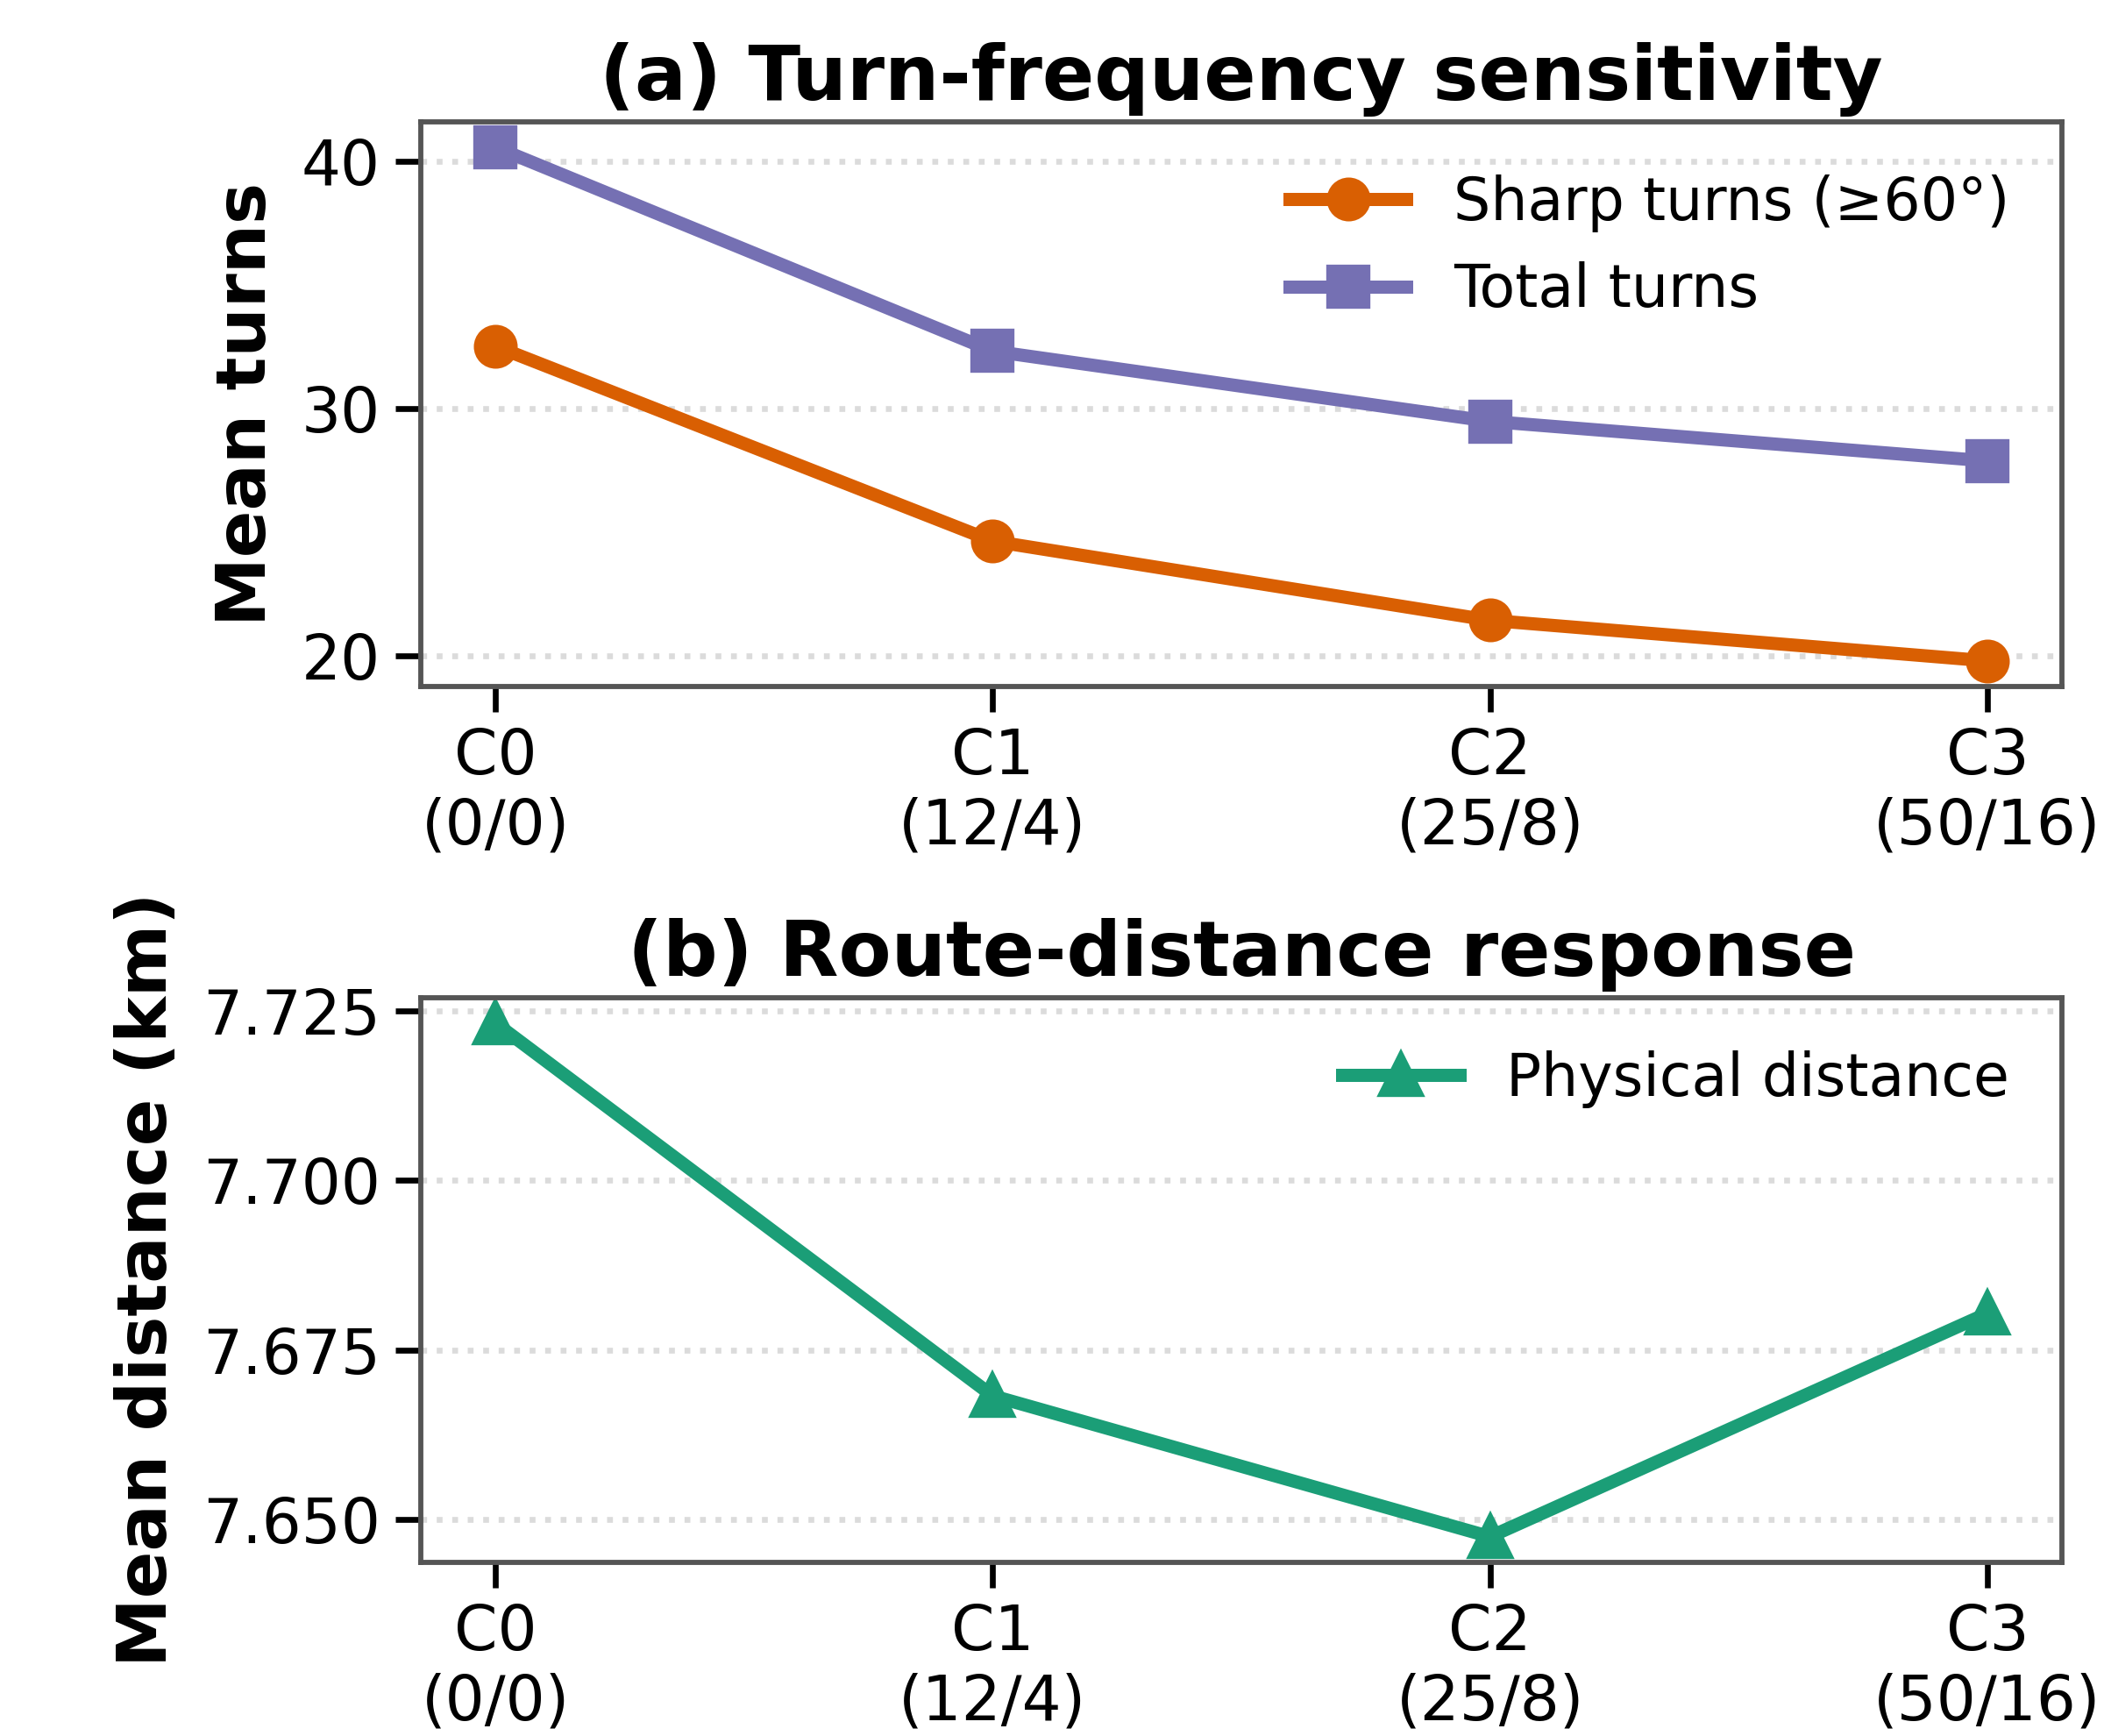
\includegraphics[width=\columnwidth]{fig3_exp_c_sensitivity.png}
\caption{Experiment C sensitivity across 25 corridors: (a) mean sharp-turn and total-turn counts under penalty tiers $C_0$ ($0/0$), $C_1$ ($12/4$), $C_2$ ($25/8$), and $C_3$ ($50/16$); (b) mean physical route distance under the same configurations.}
\label{fig:exp_c_sensitivity}
\end{figure}

\subsection{Topological Modifiers: Bridge and Roundabout Effects}

The $2\times2$ D design tests bridge (0.80) and roundabout (0.95) modifiers. Bridge activation changed routes only on OD\_04 (about -645 m) and OD\_15 (-2.15 km); 23/25 were unchanged. The D3--D4 post-hoc standardized impedance-cost difference was +120.92 (adjusted $p=0.4722$, $d_z=0.2192$). Roundabout comparisons produced no route or distance changes across 25 corridors; OD\_06 included 62.98 m of roundabout traversal. The harness did not retain configured search-objective costs; post-hoc production scoring is not a substitute.

\subsection{Primary Inferential Hypothesis Test Summary}

Table~\ref{tab:statistical_results} reports ten paired tests across six families. Eight are significant ($p_{\mathrm{adj}}\le1.5\times10^{-4}$); A1--A2 sharp turns ($p=1.000$) and D3--D4 post-hoc standardized impedance cost ($p=0.4722$) are not. Geometry/distance invariance for A1--A2 and D2--D4 is descriptive, not inferred from those tests.

\begin{table}[!t]
\caption{Paired Hypothesis Test Results ($N=25$ Corridors)}
\label{tab:statistical_results}
\centering
\footnotesize
\setlength{\tabcolsep}{1.5pt}
\renewcommand{\arraystretch}{1.08}
\begin{tabular}{@{}p{0.52in}p{0.90in}p{0.52in}p{0.25in}p{0.75in}@{}}
\hline
\textbf{Comp.} & \textbf{Outcome} & \textbf{$\Delta$ Mean} &
\textbf{$W$} & \textbf{Holm $p_{\mathrm{adj}}$} \\
\hline
$A_0$--$A_1$ & Sharp turns ($\ge60^\circ$) & $-11.08$ & $0.0$ & $\mathbf{4.5 \times 10^{-5}}$ \\
$A_1$--$A_2$ & Sharp turns ($\ge60^\circ$) & $0.00$ & $0.0$ & $1.000$ \\
$A_0$--$A_1$ & Runtime (ms) & $+41.35$ & $17.0$ & $\mathbf{1.2 \times 10^{-5}}$ \\
$A_1$--$A_2$ & Runtime (ms) & $+253.38$ & $0.0$ & $\mathbf{< 10^{-6}}$ \\
$B_0$--$B_1$ & Arterial share (\%) & $-51.21$ & $4.0$ & $\mathbf{8.4 \times 10^{-5}}$ \\
$B_0$--$B_1$ & Residential share (\%) & $+30.73$ & $9.0$ & $\mathbf{1.5 \times 10^{-4}}$ \\
$B_0$--$B_1$ & Distance (km) & $+1.028$ & $7.0$ & $\mathbf{6.8 \times 10^{-5}}$ \\
$B_0$--$B_2$ & Arterial share (\%) & $-45.51$ & $4.0$ & $\mathbf{8.4 \times 10^{-5}}$ \\
$C_3$--$C_2$ & Sharp turns ($\ge60^\circ$) & $-1.64$ & $0.0$ & $\mathbf{1.1 \times 10^{-4}}$ \\
$D_3$--$D_4$ & Post-hoc impedance cost & $+120.92$ & $0.0$ & $0.4722$ \\
\hline
\end{tabular}
\vspace{2pt}
\begin{minipage}{\columnwidth}
\scriptsize
\textit{Note:} Two-sided paired Wilcoxon tests use Pratt zero correction and Holm adjustment; bold denotes $p_{\mathrm{adj}}<0.05$. A1--A2 tests sharp turns only. D3--D4 is post-hoc standardized impedance cost, not the unretained search objective. Geometry/distance invariance statements are descriptive.
\end{minipage}
\end{table}

\section{Conclusion and Future Work}

We developed turn-aware, state-expanded $A^*$ routing with road-class impedance. Directed-edge states support turn-cost evaluation, and the Haversine heuristic scaled by 0.80 is admissible and consistent under the verified graph-specific bound $\mu(e)\ge0.80$.

Across 25 corridors, turn-aware search reduced sharp turns by 34.1\% (adjusted $p=4.5\times10^{-5}$), while median runtime rose from 154.69 to 174.93 ms. Production impedance reduced arterial exposure by 51.21 points (adjusted $p=8.4\times10^{-5}$) and increased mean physical distance by 15.53\% (adjusted $p=6.8\times10^{-5}$). C2 captured 87.1\% of the maximum observed turn reduction. Bridge effects occurred on two corridors; roundabout changes were zero across 25.

The evaluation covers one Bengaluru network and 25 corridors. No real-world journey times were measured, so travel-time reduction is unverified. Impedance is a search cost, not distance or time; sharp-turn counts do not establish safety or accident reduction. We did not calibrate weights to rider behaviour or retain Experiment D search-objective costs.

Future work includes multi-city evaluation, GPS- and rider-choice calibration, measured journey-time assessment, dynamic traffic, gradients, and vehicle-specific constraints.

\balance
\bibliographystyle{IEEEtran}
\bibliography{paper1_verified_references}

\end{document}
